\documentclass[10pt,journal]{IEEEtran}

\usepackage{graphicx}
\usepackage{amsmath}
\usepackage{booktabs}
\usepackage{hyperref}
\usepackage{xcolor}
\usepackage{caption}

\hypersetup{colorlinks=true, linkcolor=blue, urlcolor=blue, citecolor=blue}

\graphicspath{{figures/}}

\begin{document}

\title{Project Documentation: Process Maps and Literature Validation\\
\large for the Rosenthal Melt-Pool Calculator}

\author{Adeleke Olorunnisola Oyeyemi\\
\textit{Department of Mechanical Engineering, Federal University of Technology, Akure, Nigeria}\\
Source code: \url{https://github.com/Olorunnisola01/rosenthal-meltpool}\\
Interactive demo: \url{https://rosenthal-meltpool.streamlit.app}}

\markboth{Project 2 Documentation}{}

\maketitle

\begin{abstract}
This document describes Project 2 of a six-month research-preparation programme in metal additive manufacturing (AM) process modelling, building directly on Project 1 (a Python/Streamlit calculator implementing the Rosenthal moving point-heat-source solution, documented separately). Project 2 has two parts: a power-velocity parameter sweep that generates process maps for four L-PBF alloys, and a validation of the calculator's predictions against a real published single-track dataset. The validation is the more consequential result: at the source study's own assumed absorptivity, the model underpredicts every published case, and a calibration search shows this cannot be corrected by absorptivity alone for most cases. Combined with a process-map finding --- that the predicted depth-to-width ratio is exactly 0.5 everywhere, for every material, confirmed here across the full swept parameter range rather than at isolated points --- this document establishes the quantitative boundaries within which the Project 1 calculator's output should be trusted, and motivates the heat-source modelling choices for later, more physically complete work.
\end{abstract}

\section{Introduction}

Project 1 established that the Rosenthal moving point-heat-source solution predicts a melt pool whose depth is always exactly half its width, for any material or process parameters --- a mathematical identity of the model, confirmed at a handful of worked examples. Two questions follow directly from that finding, and both required going beyond single-point evaluation: does the identity hold everywhere across the process window, or only at the specific parameter combinations tested; and, more importantly, how do the model's absolute predictions compare against a real measured single-track dataset, not just against each other. This project answers both questions by (i) sweeping the calculator over a full power$\times$velocity grid for all four preset alloys, and (ii) validating predictions against a published dataset with independently measured melt-pool dimensions.

\section{Parameter Sweep Methodology}

The core package's \texttt{sweep.py} module evaluates \texttt{melt\_pool\_dimensions} at every point on a power$\times$velocity grid, holding absorptivity and preheat temperature fixed, and returns width, depth, length, and aspect ratio (depth/width) as 2D arrays. Points where the transcendental root-finder fails to converge (sub-threshold parameters that produce no melt pool at all) are recorded as \texttt{NaN} rather than raising an error, so a sweep can span parameter combinations where some points are physically sub-threshold without halting the whole grid.

For the process maps in this document, power was swept from 50 to 400~W and velocity from 200 to 2000~mm/s, each in 45 steps, at a fixed absorptivity of 0.4 and preheat of 300~K, matching the Project 1 calculator's default operating point.

\section{Process Maps}

\begin{figure}[!t]
\centering
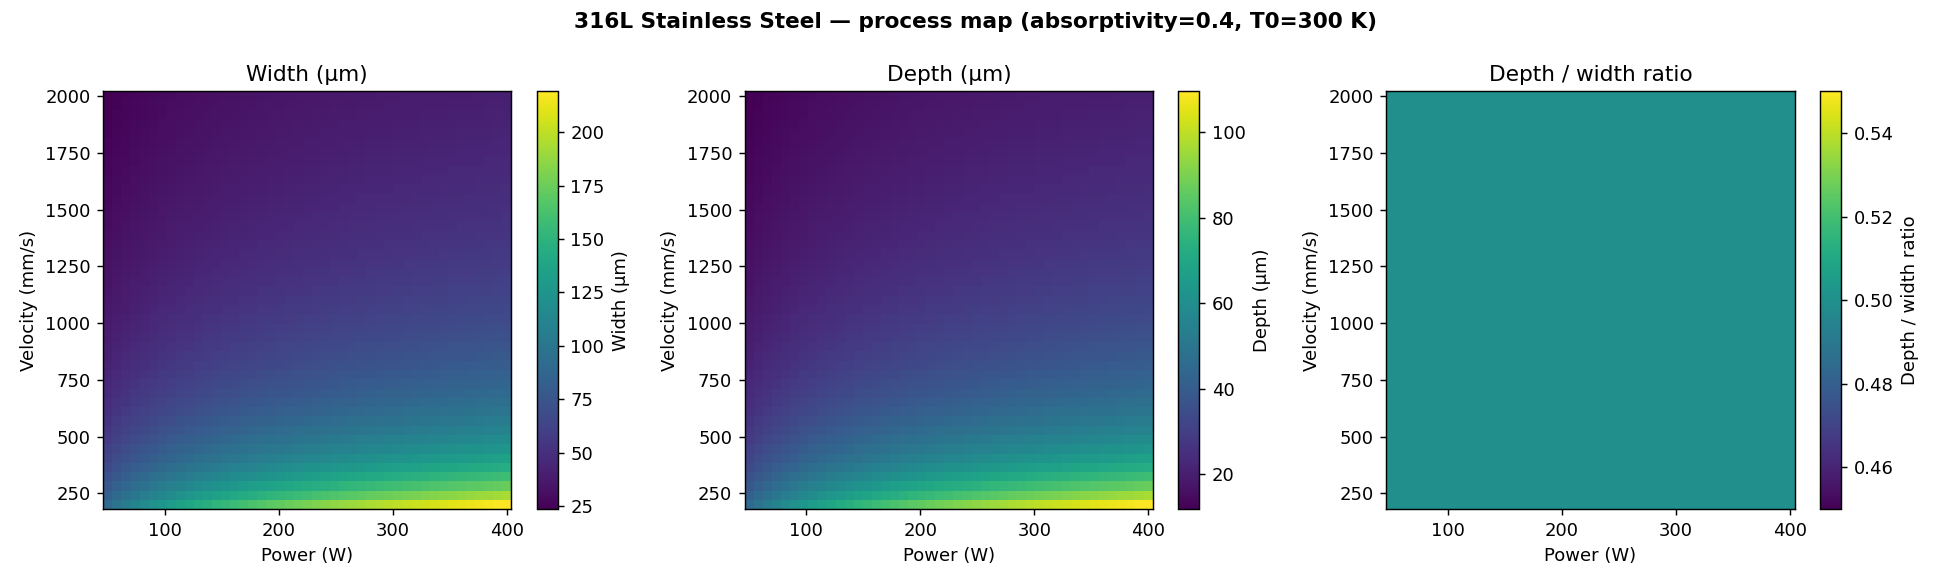
\includegraphics[width=\columnwidth]{process_map_316L.png}
\caption{316L process map: width, depth, and depth/width ratio across the full power-velocity grid. The third panel is visually uniform because it is uniform --- every point evaluates to 0.5, to within floating-point precision.}
\label{fig:map316l}
\end{figure}

\begin{figure}[!t]
\centering
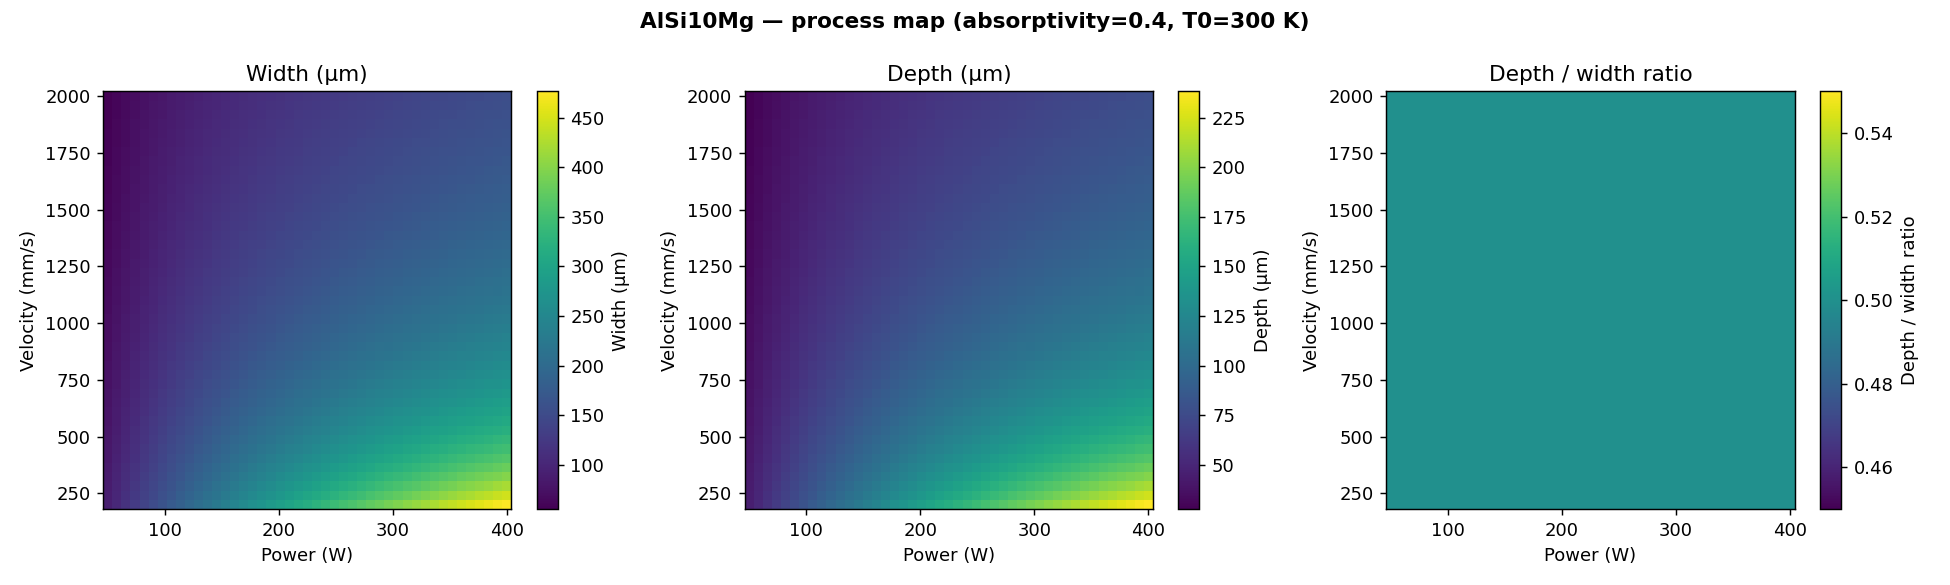
\includegraphics[width=\columnwidth]{process_map_AlSi10Mg.png}
\caption{AlSi10Mg process map at identical sweep ranges. Peak width reaches roughly 470~\textmu m, over twice 316L's roughly 220~\textmu m peak in Fig.~\ref{fig:map316l}, at identical power and velocity --- a direct visual confirmation that thermal conductivity, not process parameters, sets the overall scale of the melt pool.}
\label{fig:mapalsi}
\end{figure}

Figs.~\ref{fig:map316l} and \ref{fig:mapalsi} show the swept process maps for 316L and AlSi10Mg. Both alloys show the expected qualitative trend --- width and depth increase with power and decrease with velocity --- but the two materials occupy entirely different absolute scales, consistent with AlSi10Mg's roughly 5$\times$ higher thermal conductivity. The third panel in each figure, depth/width ratio, is the more important result: it is flat --- not approximately flat, but numerically 0.5 at every grid point tested, for both materials and across the full power-velocity range. This confirms, by direct computation rather than by the algebraic argument alone, that the semicircular cross-section identified in Project 1 is not an artifact of the specific parameter values used there; it holds everywhere this model can be evaluated. A dedicated regression test locks this property into the package's test suite across all four alloys, so any future change to the model that broke it would be caught immediately.

\section{Literature Validation}

\subsection{Dataset and Method}

Model predictions were compared against four published bare-plate single-track measurements for 316L stainless steel, from Zhang \textit{et al.} (2024) \cite{zhang2024}, Table 3. The source study reports laser power, scan velocity, measured melt-pool width, and measured melt-pool depth for each case, and states an assumed absorptivity of 0.5 and a 100~\textmu m laser spot diameter in its own numerical model. Predictions were generated with the same absorptivity (0.5) and a preheat of 300~K (room temperature, the conventional default for bare-plate experiments; not stated explicitly in the source paper).

\begin{table}[!t]
\centering
\caption{Predicted vs. measured melt-pool dimensions, Zhang et al. (2024)}
\label{tab:validation}
\begin{tabular}{@{}lrrrrrr@{}}
\toprule
Case & $P$ (W) & $v$ (mm/s) & $W_{\text{pred}}$ & $W_{\text{meas}}$ & $D_{\text{pred}}$ & $D_{\text{meas}}$ \\
& & & (\textmu m) & (\textmu m) & (\textmu m) & (\textmu m) \\
\midrule
N01 & 260 & 520 & 105.8 & 114.0 & 52.9 & 180.0 \\
N04 & 260 & 1470 & 48.7 & 94.0 & 24.4 & 61.0 \\
N05 & 260 & 2200 & 35.6 & 83.0 & 17.8 & 41.0 \\
N06 & 440 & 1470 & 54.7 & 98.0 & 27.4 & 104.0 \\
\bottomrule
\end{tabular}
\end{table}

\subsection{Results}

Table~\ref{tab:validation} gives predicted and measured width and depth for all four cases. The model underpredicts every single case, in both dimensions, ranging from a $-7.2\%$ width error (N01) to a $-73.7\%$ depth error (N06). Measured aspect ratios (depth/width) for these four cases are 1.58, 0.65, 0.49, and 1.06 respectively --- directly demonstrating the range of real melt-pool shapes the model's fixed 0.5 ratio (Section~III) cannot represent.

\subsection{Absorptivity Calibration Search}

Because absorptivity is the one input not fixed by material properties, a calibration search was run for each case: holding power, velocity, and material fixed, find the absorptivity that makes predicted width (or depth) exactly match the measured value, searching up to 500\% --- a deliberately unphysical upper bound, used to distinguish ``the guessed absorptivity was wrong'' from ``no absorptivity closes this gap.''

\begin{table}[!t]
\centering
\caption{Calibrated absorptivity search (bounds: 1\%--500\%)}
\label{tab:calibration}
\begin{tabular}{@{}lcc@{}}
\toprule
Case & Calibrated for width & Calibrated for depth \\
\midrule
N01 & 0.658 & no solution \\
N04 & no solution & no solution \\
N05 & no solution & no solution \\
N06 & no solution & no solution \\
\bottomrule
\end{tabular}
\end{table}

Table~\ref{tab:calibration} shows that depth cannot be matched for \emph{any} of the four cases at any absorptivity up to 500\%, and width can only be matched for one case (N01, at a plausible 65.8\%). For the other three cases, the gap between prediction and measurement persists even at an absorptivity five times larger than physically possible.

\subsection{Interpretation}

The predicted pool sizes in these cases (35--115~\textmu m) are the same order of magnitude as the 100~\textmu m laser spot diameter the source study reports. The point-source assumption underlying the Rosenthal solution requires the resulting pool to be much larger than the source itself; these cases sit at or below that threshold, so the assumption is not satisfied, independent of what absorptivity value is chosen. This is a more precise, falsifiable statement than the qualitative caveat given in Project 1 --- it is now backed by a specific numeric search showing where and how badly the assumption breaks down for a real dataset.

N01 is the case closest to being matched (width matchable at a plausible absorptivity), and it is also the case with the highest measured aspect ratio (1.58, i.e. keyhole-influenced) and the largest absolute pool size of the four --- consistent with the point-source assumption holding somewhat better as pool size grows relative to spot size, even though depth remains unmatched because keyhole-mode depth enhancement is outside what any conduction-only model can represent.

\section{Implications for Paper 2}

These results directly shape the analytical melt-pool modelling manuscript planned as Paper 2. The process maps (Section~III) supply the standard process-window figures expected in that paper's methodology section. The validation and calibration search (Section~IV) supply its most citable content: a quantified, falsifiable account of where and why the classical point-source model fails on real data, rather than a restatement of textbook caveats. The natural next methodological step --- not undertaken here --- is comparison against a heat-source model that removes the point-source assumption, such as a finite Gaussian surface flux or Goldak's double-ellipsoidal source \cite{goldak1984}, to test whether either closes the gap identified in Table~\ref{tab:validation} without sacrificing the closed-form speed that makes the Rosenthal model useful for process-window screening in the first place.

\section{Conclusion}

Project 2 extends Project 1's single-point calculator into a swept process-mapping tool and, more importantly, into a quantitatively validated one. Two findings carry forward into the accompanying paper: the depth/width$=0.5$ identity holds across the entire explored process window for every alloy, not just at isolated points; and a calibration search against real published data shows the model's absorptivity is not always sufficient to explain observed discrepancies, with the root cause traced to a specific, checkable condition (pool size relative to laser spot size) rather than left as an unquantified caveat.

\begin{thebibliography}{9}

\bibitem{zhang2024}
S. Zhang \textit{et al.}, ``Understanding melt pool behavior of 316L stainless steel in laser powder bed fusion additive manufacturing,'' \textit{Micromachines}, vol. 15, no. 2, p. 170, 2024, doi: 10.3390/mi15020170.

\bibitem{goldak1984}
J. Goldak, A. Chakravarti, and M. Bibby, ``A new finite element model for welding heat sources,'' \textit{Metallurgical Transactions B}, vol. 15, no. 2, pp. 299--305, 1984.

\end{thebibliography}

\end{document}
